% vim: set tw=78 sts=2 sw=2 ts=8 aw et ai:
\documentclass[12pt]{article}

\usepackage[paper=a4paper, top=2cm, bottom=3cm, left=2.5cm, right=2.5cm]{geometry}

\usepackage{ucs}
\usepackage[utf8x]{inputenc}
\usepackage[english]{babel}
%\usepackage{hyperref}	  % use \url{http://$URL} or \href{http://$URL}{Name}
\usepackage{underscore}	  % underscores need not be escaped
\usepackage{subfigure}
\usepackage{verbatim}
\usepackage{float}
\usepackage{array}
\usepackage{parskip}
\usepackage{placeins}


% Support for including graphics
\usepackage{graphicx}
\DeclareGraphicsExtensions{.pdf,.png,.jpg}

\title{Galileo High Accuracy Service Receivers Using FPGA and DSP}

\author{Andrei Ursulean\\
Faculty of Electronics, Telecommunications and Information Technology\\
University POLITEHNICA of Bucharest\\
Splaiul Independenței 313, Bucharest, Romania, 060042 \\
\emph{andrei.ursulean@stud.aero.upb.ro}}

\date{\today}

\begin{document}

\maketitle

\begin{abstract}
% vim: set tw=78 sts=2 sw=2 ts=8 aw et ai:

First developed in the 20th century as a military technology, Global Navigation Satellite Systems (GNSS) soon found numerous civilian applications. Nowadays, GNSS has become a part of our everyday life and it is an enabling technology in many areas, from consumer electronics, to aviation, transportation, agriculture and geomatics. Initially, the system offered an accuracy of about five meters, but algorithms and technologies for improving the accuracy have been developed and current GNSS receivers provide a precision of less than 30 centimeters with professional-grade equipment being able of sub-milimeter accuracy. With the emergence of autonomous cars, unmanned vehicles and robotics, the GNSS market is only expected to grow even further. Galileo, the European Union civilian GNSS, aims to provide higher-precision capabilities for free. In this work we will explore current state-of-the-art solutions for GNSS signals decoding based on Software Defined Radio, DSP and FPGA and corrections applications for high-accuracy positioning.

\textbf{Keywords:} GNSS, Galileo, PPP, SDR, FPGA, DSP
\end{abstract}

\section{Introduction}
\label{sec:introduction}
% vim: set tw=78 sts=2 sw=2 ts=8 aw et ai:

Global Navigation Satellite System (GNSS) positioning relies on computing the pseudoranges between the receiver and the satellite. The pseudoranges are calculated by measuring the transmitting time of the signals emitted by the satellites and multiplying with the speed of light. Ranges to four satellites and their orbital positions are required for computing the positioning solution. Since there are many possible inaccuracies in the measuring chain of the propagation time, we use the term pseudoranges for these distances to the satellites.

The first GNSS receivers consisted of large analog equipment, back in the 1970s when GNSS was a military-only technology\cite{receivers}. Now, due to their popularity and wide area of applications, they are mostly miniaturized platforms implemented on microprocessors, Integrated Circuits (IC), FPGAs, DSPs\cite{receivers}. They are found in almost all mobile phones. Usually, GNSS receivers are implemented in hardware, that means it is a dedicated chip designed specifically for this purpose. However, with the development of software defined radio (SDR) technologies, software GNSS receiver becoming increasingly popular because they have the advantage of increased flexibility.

The European Commission decided to offer the Galileo High Accuracy signal for free in order to allow the industry and the community to innovate both emerging and estabilished markets\cite{galileoHasPolicy}. The Galileo Commercial Service, which aims to provide precise point positioning will broadcast corrections over the E6B signal while The E6C signal will be used for authentication\cite{e6breceiver}. Most aspects of the signals are public and can be found in the Galileo Signal in Space Interface Control Document \cite{galileoSisIcd}.

In this work, we will present the state-of-the-art of GNSS accuracy and high accuracy positioning methods, then we look at the Galileo HAS and Galileo E6 signal and finally, we review some papers presenting GNSS receiver implementations.


% \section{GNSS}
% \label{sec:gnss_intro}
% \input{src/gnss_intro}

\section{GNSS Accuracy}
\label{sec:gnss_accuracy}
Since the beginning of the GNSS technologies, the accuracy has improved to around 1-meter precision\cite{galileoHasPolicy}. The first step to improve the accuracy for the general public was to remove the GPS selective availability in May 2000\cite{galileoHasPolicy}. Afterwards, the accuracy was improved by reducing the error in orbits calculation, ionospheric propagation models and clocks\cite{galileoHasPolicy}. Another major improvement was the development of satellite-based augmentation systems (SBAS). These augmentation systems were developed for the requirements of civil aviation and they compute positioning integrity and transmit satellite and ionospheric corrections\cite{galileoHasPolicy}. Examples of these systems are the American WAAS and the European EGNOS. These systems however, only have regional coverage area.

To further improve the accuracy, Differential GNSS (DGNSS) and Real-time Kinematic (RTK) techniques have been developed. Differential GNSS works by measuring the most of errors in a nearby station\cite{galileoHasPolicy}. For sub-decimeter-level positioning accuracy, it is required to use carrier phase measurements. RTK is similar to DGNSS, but applied to carrier phase \cite{galileoHasPolicy}. The differential GNSS techniques requires a second nearby station with a known position, therefore it is limited to an area of tens of kilometers\cite{galileoHasPolicy}.

On the other hand, Precise Point Positioning(PPP) provides centimeter-level accuracy and requires only one receiver. This technique involves a stream of absolute corrections to the GNSS Receiver. Ionospheric errors can be corrected by using the propagation of multiple signals on different frequencies. PPP techniques are still under development. Initial methods converged to a solution in hours, while recent developments have much faster convergence time\cite{galileoHasPolicy}\cite{instantPPP}. 

\section{PPP Improvements}
\label{sec:gnss_ppp}
In contrast to RTK, one of the inconveniences of PPP is the convergence time required for computing a position solution. However, a solution to reduce the convergence time is o use multiple systems with multiple carrier frequencies\cite{instantPPP}. GNSS receivers can compute the distance to the satellite based on code measurement or phase measurements. Carrier phases can be measured to precision of milimeters while code pseudoranges can be measured to decimeters. The inconvenience with carrier phase measurements is that the receiver must solve the ambiguity, i.e. the number of wavelengths the signal has travelled from the satellite to the receiver. Solving this ambiguity enables very precise positioning, centimeter-level or even better. 

Most of the techniques using carrier phase measurements are based on Differential GNSS when a reference station aids a rover in determining the position\cite{instantPPP}. Even though PPP does not require a reference station, its main issue remains the long convergence time, this is why until recently, instantaneous centimeter level positioning always involved RTK. In \cite{instantPPP}, the authors state that by using signals from multiple systems with multiple carrier frequencies, their system can achieve centimeter level PPP instantaneously. 

The GNSS community has tried to solve the issues of RTK and PPP, the former is constrained to within a few kilometers of the base station while the latter has a convergence time in the order of hours and is not usable for instantaneous positioning. By providing code and carrier phase corrections, the PPP with ambiguity resolution (PPP-AR) method was developed. However, this method is still not as fast as RTK\cite{instantPPP}. Afterwards, precise atmospheric information has been included in the corrections and a unification of PPP and RTK was obtained in the PPP-RTK method. This method allows global precise positioning with rapid positioning while the receiver is in the coverage area of the reference station \cite{instantPPP}.

The recent GNSS satellites launched in orbit transmit signals on multiple frequencies. All the Galileo and BeiDou satellites use triple-frequency signals\cite{instantPPP}. Since the European Union offered the high accuracy signal at no cost in 2018, the E6 signal is transmitted by 14 Galileo satellites and can be tracked by GNSS receivers\cite{instantPPP}.

\begin{figure}[h]
\centering
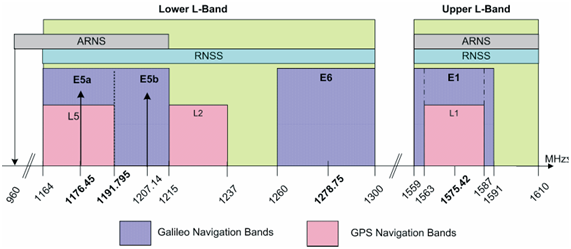
\includegraphics{img/Galileo_Frequency_Plan.png}
\caption{Galileo Frequency Plan, Source:\cite{galileoSisIcd}}
\label{fig:galileo_frequency_plan}
\end{figure}

Figure \ref{fig:galileo_frequency_plan} presents the frequencies used by GPS and Galileo. Using multiple frequencies allows phase measurements without ionosphere errors\cite{instantPPP}. The Galileo E6 signal enables instantaneous convergence for PPP-AR\cite{instantPPP}.

The GNSS receiver presented in \cite{instantPPP} uses E1, E5a, E5b and E6 signals received from one Galileo satellite to compute the ionosphere-free pseudorange, ionospheric delay and four carrier phase ambiguities\cite{instantPPP}. The Galileo E5 could also be used, however, its frequency is so close to E5a and E5b signals that its contribution is negligible\cite{instantPPP}.

\begin{table}[h!]
\centering
\begin{tabular}{|c|c|c|}
    \hline
    System & Frequencies & Range (meters) \\
    \hline
    Galileo & E1, E5a, E5b & 0.416 \\
    \hline
    Galileo & E1, E5a, E6 & 0.193 \\
    \hline
    Galileo & E1, E5b, E6 & 0.268 \\
    \hline
    Galileo & L1, L2, L5 & 0.298 \\
    \hline
\end{tabular}
\caption{Precision for three frequency single satellite configurations. Source: \cite{instantPPP}}
\label{table:20}
\end{table}

In table \ref{table:20} we can observe the precision of positioning that can be obtained in \cite{instantPPP} using 3 different frequency signals. The E1-E5a-E6 configuration has the best result and we observe that the frequency spacing is important for positioning performance.
 
\section{Galileo High Accuracy Service}
\label{sec:galileo_has}
As seen in the previous chapter, high accuracy applications are under continuous development. There are multiple options for free and public high accuracy corrections\cite{galileoHasPolicy}. Some examples from \cite{galileoHasPolicy} are:
\begin{itemize}
    \item Japanese QZSS is free over Japan. It provides centimeter-level accuracy
    \item European Galileo, Chinese Beidou and Russian GLONASS aim to provide similar accuracy for free in the upcoming years.
    \item Australia is developing the National Positioning Infrastructure Capability (NPIC) for 3-centimeters accuracy.
    \item International GNSS Service (IGS) provides high accuracy data for free.
    \item National and regional authorities which intend to provide high accuracy data for free.
\end{itemize}

Galileo High Accuracy Service (HAS) aims to provide PPP corrections for free, worldwide, via satellite links. According to \cite{galileoHasPolicy}, some characteristics of Galileo HAS are:
\begin{itemize}
    \item High Accuracy corrections transmitted for free, using an open standard format via the new Galileo E6-B signal with the possibility to transmit via terrestrial networks at the same time.
    \item The navigation messages will contain error corrections for satellite orbits, clocks, code and phase biases.
    \item The system will focus on Galileo and in the future it is possible to be extended to other GNSS.
    \item The service will be global with the possibility to include a regional augmentation over EU for ionospheric corrections.
    \item The positioning accuracy will be less than two decimeters.
\end{itemize}

The corrections will be included in the Galileo E6-B signal and will be transmitted by around $80\%$ of the satellites\cite{galileoHasPolicy}. The signal characteristics are presented in table \ref{table:1}
\begin{table}[h!]
\centering
\begin{tabular}{| m{15em} | m{20em} |}
    \hline
    \multicolumn{2}{|c|}{Signal and Data features} \\
    \hline
    Frequency & 1278.75 MHz \\
    \hline
    Signal & E6B \\
    \hline
    Min. Power & -158 dBW \\
    \hline
    Chip Rate & 5.115 Mcps \\
    \hline
    Code Length & 1 ms \\
    \hline
    Symbol Rate & 1000 sps \\
    \hline
    Data Rate & 492 bps \\ 
    \hline
    HA Data Rate & 448 bps \\
    \hline
    Data Coding & FEC as per Galileo OS ICD + interleaving $123 \times 8$ \\
    \hline
    Spreading Code Encryption & No \\
    \hline
    Data & Orbit and clock corrections, code and phase biases, flags, ionospheric information \\
    \hline
\end{tabular}
\caption{Galileo HAS E6B signal and data features. Source: \cite{galileoSisIcd}}
\label{table:1}
\end{table}

\subsection{Galileo E6 Signals}
\label{subsec:e6signals}

Paper \cite{e6breceiver} presents the E6B and E6C signals used in the Galileo HAS. The E6B and E6C signals are already being transmitted by satellites in orbit. The E6B signal will provide 492 bits per second per satellite of PPP corrections. This band allocation is new for GNSS and some reception and demodulation difficulties can be expected due to interference with radio amateurs, radars and due to the high bit-rate of the transmission\cite{e6breceiver}. However, This new band also comes with many new opportunities. The frequency is well separated from both E1 and E5 and the high bandwidth allows the transmission of corrections. The importance of frequency separation for ionosphere error elimination has been presented in \cite{instantPPP}.

The E6 Galileo signal is spread in two components \cite{e6breceiver}:
\begin{itemize}
    \item The data component (E6B), a modulo-two addition of FEC encoded data stream modulated by Binary Phase Shift. Keying (BPSK)
    \item The Pilot component (E6C), modulo-two addition of a code sequence with BPSK modulation.
\end{itemize}

\begin{table}[h!]
\centering
\begin{tabular}{| c | c | c |}
    \hline
    & E6B & E6C \\
    \hline
    Component & Data & Pilot \\
    \hline
    Carrier Frequency & 1278.75 Mhz & 1278.75 Mhz \\
    \hline
    Signal Polarization & RHCP & RHCP \\
    \hline
    Modulation & BPSK & BPSK \\
    \hline
    Chip Rate & 5.115 Mcps & 5.115 Mcps\\
    \hline
    Primary Code Length & 5115 chips & 5115 chips \\
    \hline
    Secondary Code Length & N/A & 100 chips \\
    \hline
    Secondary Code Length & N/A & 100 ms \\
    \hline
    Symbol Rate & 1000 sps & N/A \\
    \hline
    Data Rate & 492 bps & N/A\\
    \hline
    Data interleaving & $123 \times 8$ & N/A\\
    \hline
    Spreading Code Encryption Capability & Yes & Yes \\
    \hline
    Power Sharing & 50\% & 50 \% \\
    \hline
    Received minimum power & -155 dBW & -155 dBW \\
    \hline
\end{tabular}
\caption{Galileo E6 Properties. Source: \cite{e6breceiver}}
\label{table:2}
\end{table}

\begin{figure}[h]
\centering
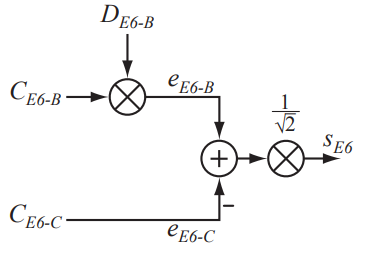
\includegraphics[scale=0.7]{img/signal_generation.png}
\caption{E6 Signal Generation, Source:\cite{e6breceiver}}
\label{fig:signal_generation}
\end{figure}

The E6 signal characteristics can be found in table \ref{table:2}. The signal generation diagram is presented in figure \ref{fig:signal_generation}. Before the data signal enters the mixer, a logic 0 bit is mapped to +1 signal level and a logic 1 bit is mapped to -1 signal level\cite{e6breceiver}.

\subsection{Galileo E6-B Data Structure}
\label{subsec:e6data}

As presented here, the data component of the E6 signal is transmitted via the E6B signal. In table \ref{table:2} we can see that the data is sent at 1000 symbols per second. Out of these 1000 symbols, the first 16 are the synchronization pattern. The remaining 984 symbols encode 492 data bits using Forward Error Correction (FEC). The data bits contain the PPP corrections. The corrections data will rely on external providers \cite{e6breceiver}. 



\FloatBarrier

\section{GNSS Receivers}
\label{sec:gnss_receivers}
So far we have looked at different GNSS services and signals. However, we have no influence over the space and ground segment of GNSS. The only segment that we can work on and improve is the GNSS receiver segment. The receiver is responsible for processing the signal broadcasted by the satellites and computing the position, velocity and time (PVT)\cite{receivers}. Another major task of the receivers is to acquire and track the satellite signals since the satellites are always in motion and they do not stay in view for long\cite{receivers}. Briefly, a receiver computes the propagation time and multiplies it with speed of light. This produces a very rough estimate of the distance due to the all the errors in the propagation of the signal. However, using four pseudoranges, the navigation solution can be computed. 

Most of the current GNSS receivers are hardware receivers. This means that they are a dedicated piece of hardware equipment designed specifically for this purpose. This has the advantages that it takes the computing load off other equipment and since they optimized for this specific application they are more power efficiency, which is desirable in embedded applications. The hardware approach for GNSS receiver is based mostly on FPGA and ASIC chips\cite{dsp_receiver}. The inconvenience with hardware receivers is that they lack flexibility. When new GNSS signals or constellations are developed, hardware receivers are very difficult to upgrade. The growth in computing power and accessibility for embedded CPUs contributed to the gain in popularity of software GNSS receivers. In paper \cite{dsp_receiver}, the authors present a Digital Signal Processor (DSP) based GNSS receiver for multiple constellations.

The techniques used in software GNSS receivers are inspired from software defined radio (SDR) technology. SDR is very popular in the scientific community due to its flexibility, allowing many experiments to be performed using a single piece of equipment. Usually for SDR applications, the signal is down-converted to a lower frequency then it is sampled using an analog-to-digital converter (ADC) and processed by software running on a general purpose CPU. A GNSS receiver must also perform acquisition, tracking and solving for the PVT solution\cite{dsp_receiver}. Software receiver applications can be performed either on a general purpose PC or on a DSP. 

\subsection{DSP Real-time Multichannel Receiver\cite{dsp_receiver}}
\label{subsec:dsp_recv}

The receiver proposed in \cite{dsp_receiver} uses an GP2015 RF front-end chip to down-convert the signal to an intermediate frequency. The signal is then sampled by the ADC and transmitted to a Texas Instruments TMS320C6416 DSP chip which will perform all the necessary operations: acquisition, tracking and positioning. The chip was selected by the authors to have enough processing power for supporting multiple constellations. Since the navigation signal is below the noise level, the ADC precision is not significant\cite{dsp_receiver}. For this reason, the authors have used 1bit or 2 bit quantization.

\begin{figure}[h]
\centering
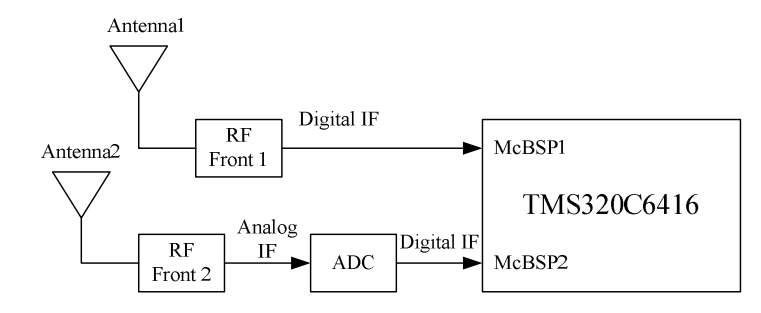
\includegraphics[width=\textwidth]{img/dsp_gnss_signal.png}
\caption{DSP GNSS Receiver Signal Input, Source:\cite{dsp_receiver}}
\label{fig:galileo_frequency_plan}
\end{figure}

Since many satellite navigation systems use similar principles, some software modules can be reused on different signal sources. For example, in GPS and Galileo, the positioning and acquisition modules are common\cite{dsp_receiver}. The software architecture proposed by \cite{dsp_receiver} contains three main tasks: tracking task, positioning task and acquisition task, in the order of task priority. Because of the multi-constellation support, two tracking tasks will run at the same level of priority. In the end we can see that the receiver proposed by the authors of \cite{dsp_receiver} can track 10 satellites in single constellation mode and 5 satellites in two constellations mode.

\subsection{MBOC Receiver\cite{ref_station_receiver}}
\label{subsec:mboc_recv}

The paper \cite{ref_station_receiver} presents the designing of a reference station receiver for Galileo and GPS. Since this receiver is designed as a reference station for the mission segment, it requires high quality measurements for pseudorange, carrier phase and status information in order to compute the errors and the integrity of navigation signal\cite{ref_station_receiver}. The work of the authors is based on their previous experience with Galileo and GNSS at Thales Alenia Space. This station is designed to work on the following signals\cite{ref_station_receiver}:

\begin{itemize}
    \item GPS L1/L2
    \item Galileo E1B, E1C, E6B, E6C, E5a, E5b, E5AltBOC
    \item Giove E1A and E6B
\end{itemize}

\begin{figure}[h]
\centering
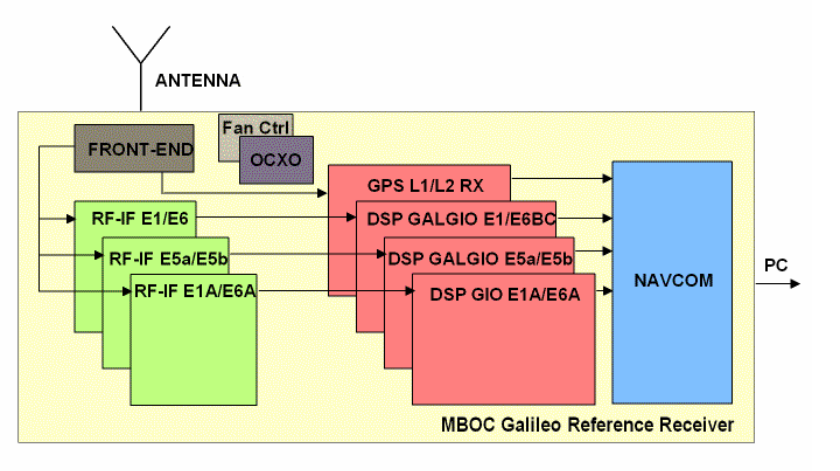
\includegraphics[width=\textwidth]{img/mboc_architecture}
\caption{MBOC Receiver Architecture, Source:\cite{ref_station_receiver}}
\label{fig:mboc_architecture}
\end{figure}

The architecture proposed by \cite{ref_station_receiver} can be seen in Figure \ref{fig:mboc_architecture}. It is composed of a high-performance multi-band active GNSS antenna with filters and low noise amplifier, RF front-end for further amplification and filtering, RF down-converters, three Digital Signal Processors and a Navigation \& Communication Processor which implements the navigation processing. 

The RF part of the system are responsible for splitting of the signal from the antenna to lines corresponding to all different carriers in the signal, feeding DC bias for the active antenna and compensating for the cable losses. The next part is the intermediate frequency down converter which also performs automatic gain control (AGC)\cite{ref_station_receiver}. 

\begin{figure}[h]
\centering
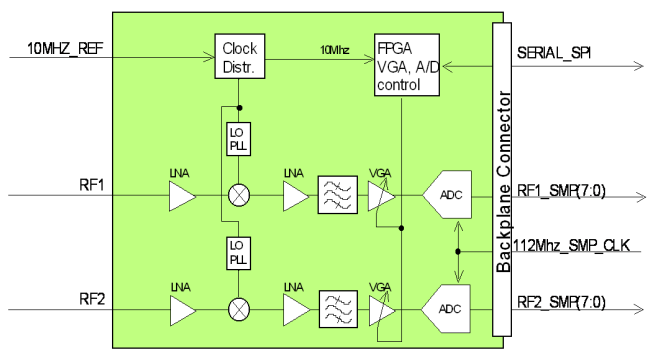
\includegraphics[width=\textwidth]{img/rf_if_block}
\caption{RF-IF Board Block Diagram, Source:\cite{ref_station_receiver}}
\label{fig:rf_if_block_diagram}
\end{figure}

The DSP Block is responsible for\cite{ref_station_receiver}:
\begin{itemize}
    \item Acquisition and tracking of signal.
    \item Measuring pseudorange, carrier phase doppler and carrier-to-noise ratio.
    \item Decoding navigation messages.
    \item performing satellite prediction and selecting satellite tracking channels based on the predictions.
    \item Managing RF-IF AGC.
\end{itemize}

The receiver channels are implemented in FPGA chips based on a Thales Alenia Space proprietary technology called GALVANI\cite{ref_station_receiver}. The signal processing chain is shared between the Galvani FPGAs and a digital signal processor. The Galvani hardware is composed of channels, also called Single Frequency Channels (SFC)\cite{ref_station_receiver} which consist in a matrix of signal processing elements. The SFC implements all the necessary modules for demodulating the GNSS signal. The Galvani cores includes\cite{ref_station_receiver}:

\begin{itemize}
    \item IF Real to Complex Converter (RCC) which takes at it's input 3 to 8 bits digitized samples and performs filtering, down-conversion to baseband, sample decimation.
    \item Code and Carrier tracking
    \item Time base generator for synchronizing with other external devices.
    \item Viterbi decoder
    \item DSP interface
\end{itemize}

\begin{figure}[h]
\centering
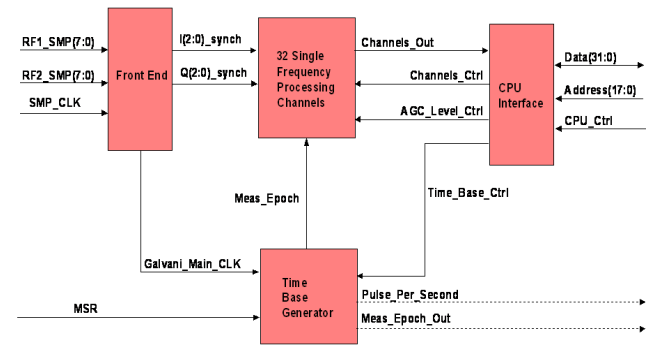
\includegraphics[width=\textwidth]{img/galvani_core}
\caption{RF-IF Board Block Diagram, Source:\cite{ref_station_receiver}}
\label{fig:galvani_core}
\end{figure}

The next component of the receiver is the Navigation and Communication Subsystem which is responsible for taking the observables processed by the DSP subsystem and computing the navigation solution and then comunicating the solution to the user, in this case it is connected to a computer \cite{ref_station_receiver}. The NavCom board is based on the Texas Instruments digital signal processor, the TMS320C6713, which is similar to the DSP model used by the authors in \cite{dsp_receiver}.

The testing performed by the authors in \cite{ref_station_receiver} shows that the reference receiver are compliant with the interference tests required for Galileo Sensor stations. In the end of the article the authors also propose a novel proprietary technique for E1 and E6 signals tracking called "Mirror rotation"\cite{ref_station_receiver}. 

\subsection{IFEN E6-B/C Receiver\cite{e6breceiver}}
\label{subsec:e6b_recv}
The authors of paper \cite{e6breceiver} present the development and testing of an E6-B/C signal GNSS receiver. This receiver is based on work done by the German company IFEN GmbH. The receiver is based on FPGA and supports multiple constellations and multiple frequencies with 50 MHz bandwidth. The receiver also incorporates two Arm Cortex A8 processors running embedded Linux \cite{e6breceiver}. The receiver support four channel high-speed ADC for signal sampling. It includes a high speed USB3 interface that can output the complex baseband signal stream to a computer. The baseband signal is the pre-processed by other FPGAs. The signal stream is then processed by software running on the Cortex A8 processors \cite{e6breceiver}.

\begin{figure}[h]
\centering
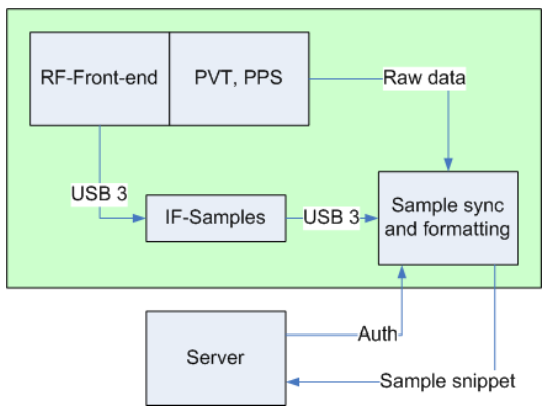
\includegraphics[scale=0.7]{img/e6b_architecture.png}
\caption{IFEN Receiver Architecture, Source:\cite{e6breceiver}}
\label{fig:e6b_architecture}
\end{figure}

The authors of \cite{e6breceiver} performed several tests in order to asses the performance of the receiver. The signal processing test result have been performed with a signal generator and the results are presented in Table \ref{table:3}. The test results using the both signal simulator and real signals are good and correspond to the theoretical expectations.

\begin{table}[h!]
\centering
\begin{tabular}{| m{12em} | m{12em} | m{12em}|}
    \hline
    Test & Description & Metric/Criteria \\
    \hline
    Multi-Signal  & Acquire and track GPS L1 and L2P, Galileo E1, E5a, E5b, E6 & All signals acquired and tracked, PVT is obtained for all signals \\
    \hline
    E6 encrypted code & Acquire and track spreading code encrypted E6 signal with key change & Tracking of encrypted signal; maintain C/N0 during key change \\
    \hline
    Signal sensitivity & Acquire and track weak signals & Tong acquisition on 34dBHz, Tracking on 28dBHz \\
    \hline
    Cold/Warm start acquisition & Measure the acquisition time & Acquisition time in line with Tong search time \\
    \hline
    Measurement Quality & Check tracking observation tracking noise vs. expectations & Tracking code range/carrier range noise in line with theory \\
    \hline
    Interference handling & Show pulse blanker and spectral filter performance & Recovery of signal when interference mitigation enabled \\
    \hline
    SAS & Test the Signal Authentication Sequences approach & Provision of correlation values when using primary code as signal sequence \\
    \hline
    RPA & Remote Processing Authentication sample collection & Check if correlation in samples is at zero code phase \\
    \hline
    
\end{tabular}
\caption{Receiver Signal Processing Tests. Source: \cite{e6breceiver}}
\label{table:3}
\end{table}
\FloatBarrier

\section{Conclusions and Further Work}
\label{sec:conclusion}
% vim: set tw=78 sts=2 sw=2 ts=8 aw et ai:
In this work we have seen the current status and the future directions of high accuracy positioning. We explored the Galileo E6 signal which will transmit error corrections for PPP algorithms and we have looked at state of the art GNSS receivers. The positioning accuracy has significantly improved and Galileo E6B is expected to provide a 20-centimeter positioning accuracy. This is suitable for most of the applications, however some professional users may require even better precision for which they will have to acquire corrections from a professional provider.
Regarding GNSS receivers, they have miniaturized and are present in many embedded devices and the majority of smartphones. We can see that most of the architectures use FPGAs for signal conditioning and DSP for signal processing and navigation solution computation. Also, DSP frequencies are quite high, in the range of GHz. Software GNSS receivers are becoming increasingly popular due to the accessibility of high performance, low power CPU and the need for flexibility and upgradeability of new GNSS receivers.

\section{Documentation Process}
\label{sec:documentation}
According to the Systematic State-of-the-Art Review Methodology, a list of keywords was compiled. The list is \emph{GNSS, Galileo, PPP, SDR, FPGA, DSP, SIS, HAS}. From these, a list of papers was selected. The following papers have been reviewed in this work.

\begin{itemize}
    \item \cite{instantPPP} in Section \ref{sec:gnssppp}
    \item \cite{galileoHasPolicy} in Section \ref{sec:gnssaccuracy} and Section \ref{sec:galileohas}
    \item \cite{e6breceiver} in Section \ref{subsec:e6brecv} and Sections \ref{subsec:e6signals} and \ref{subsec:e6data}
    \item \cite{refstationreceiver} in Section \ref{subsec:mbocrecv}
    \item \cite{dspreceiver} in Section \ref{subsec:dsprecv}
\end{itemize}

\bibliographystyle{abbrv}
\bibliography{ref}

\end{document}
